\chapter{Développements algorithmiques}
\label{chap:developpements}

Ce chapitre expose les modifications faites dans le logiciel Proteus et dans Xplor pendant la préparation de cette thèse. Xplor est un logiciel conçu pour la biologie structurale développé à l'origine par Axel T. Brünger à l'université de Yale \cite{Xplor}. Il propose un langage de script permettant d'exploiter ses fonctionnalités. Pour adapter Xplor au CPD nous y ajoutons la gestion de jeux de coordonnées multiples (rotamères) pour chaque résidu. Plusieurs modèles de solvant implicite ont également été ajoutés.

Le REMC est par nature un algorithme parallèle, nous présentons l'implémentation de cet algorithme dans proteus avec notre gestion du parallélisme. Le schéma proposé par Metropolis et Hasting constitue un cadre général dans lequel il est possible d'adapter les probabilités utilisées au système à étudier. Nous expliquons comment le critère d'acceptation a été amélioré en tenant compte de la spécificité de notre modèle et de nos objectifs. Enfin sont présentées quelques nouvelles fonctionnalités dans proteus: un système de pondération pour le choix des positions à modifier, un contrôle du taux de mutations et de changements de rotamères, une gestion dynamique de la mémoire en fonction du fichier de configuration et un système de création de labels qui simplifie la configuration.  


\section{Les Modèles }

Proteus, lors de la préparation du système, place chaque chaîne latérale possible aux différentes positions de la chaîne polypeptidique selon la librairie de rotamères de Tuffery. Ces placements sont utilisés à de nombreuses reprises pendant le calcul des énergies d'interactions. Xplor ne permettait qu'une gestion de quatre jeux de coordonnées pour une chaîne latérale simultanément. Cela oblige l'utilisation de nombreux fichiers pour stocker l'ensemble des jeux de coordonnées. Afin de remédier à ce problème, nous modifions le code source d'Xplor pour y introduire deux nouvelles notions. Une \og resclass \fg identifie un résidu par un triplet composé du \og resid \fg, du \og resname\fg et du \og segid \fg. Ces trois notions existent dans le format PDB et Xplor. Ils représentent respectivement la position dans une chaîne polypeptidique, le type d'acide aminé, le segment ou molécule à laquelle appartient le résidu. Un \og modèle \fg est un jeu de coordonnées d'une resclass. Une resclass peut avoir plusieurs modèles.
   \begin{figure}[!htbp]
     \centering
     \begin{tabular}{c}
       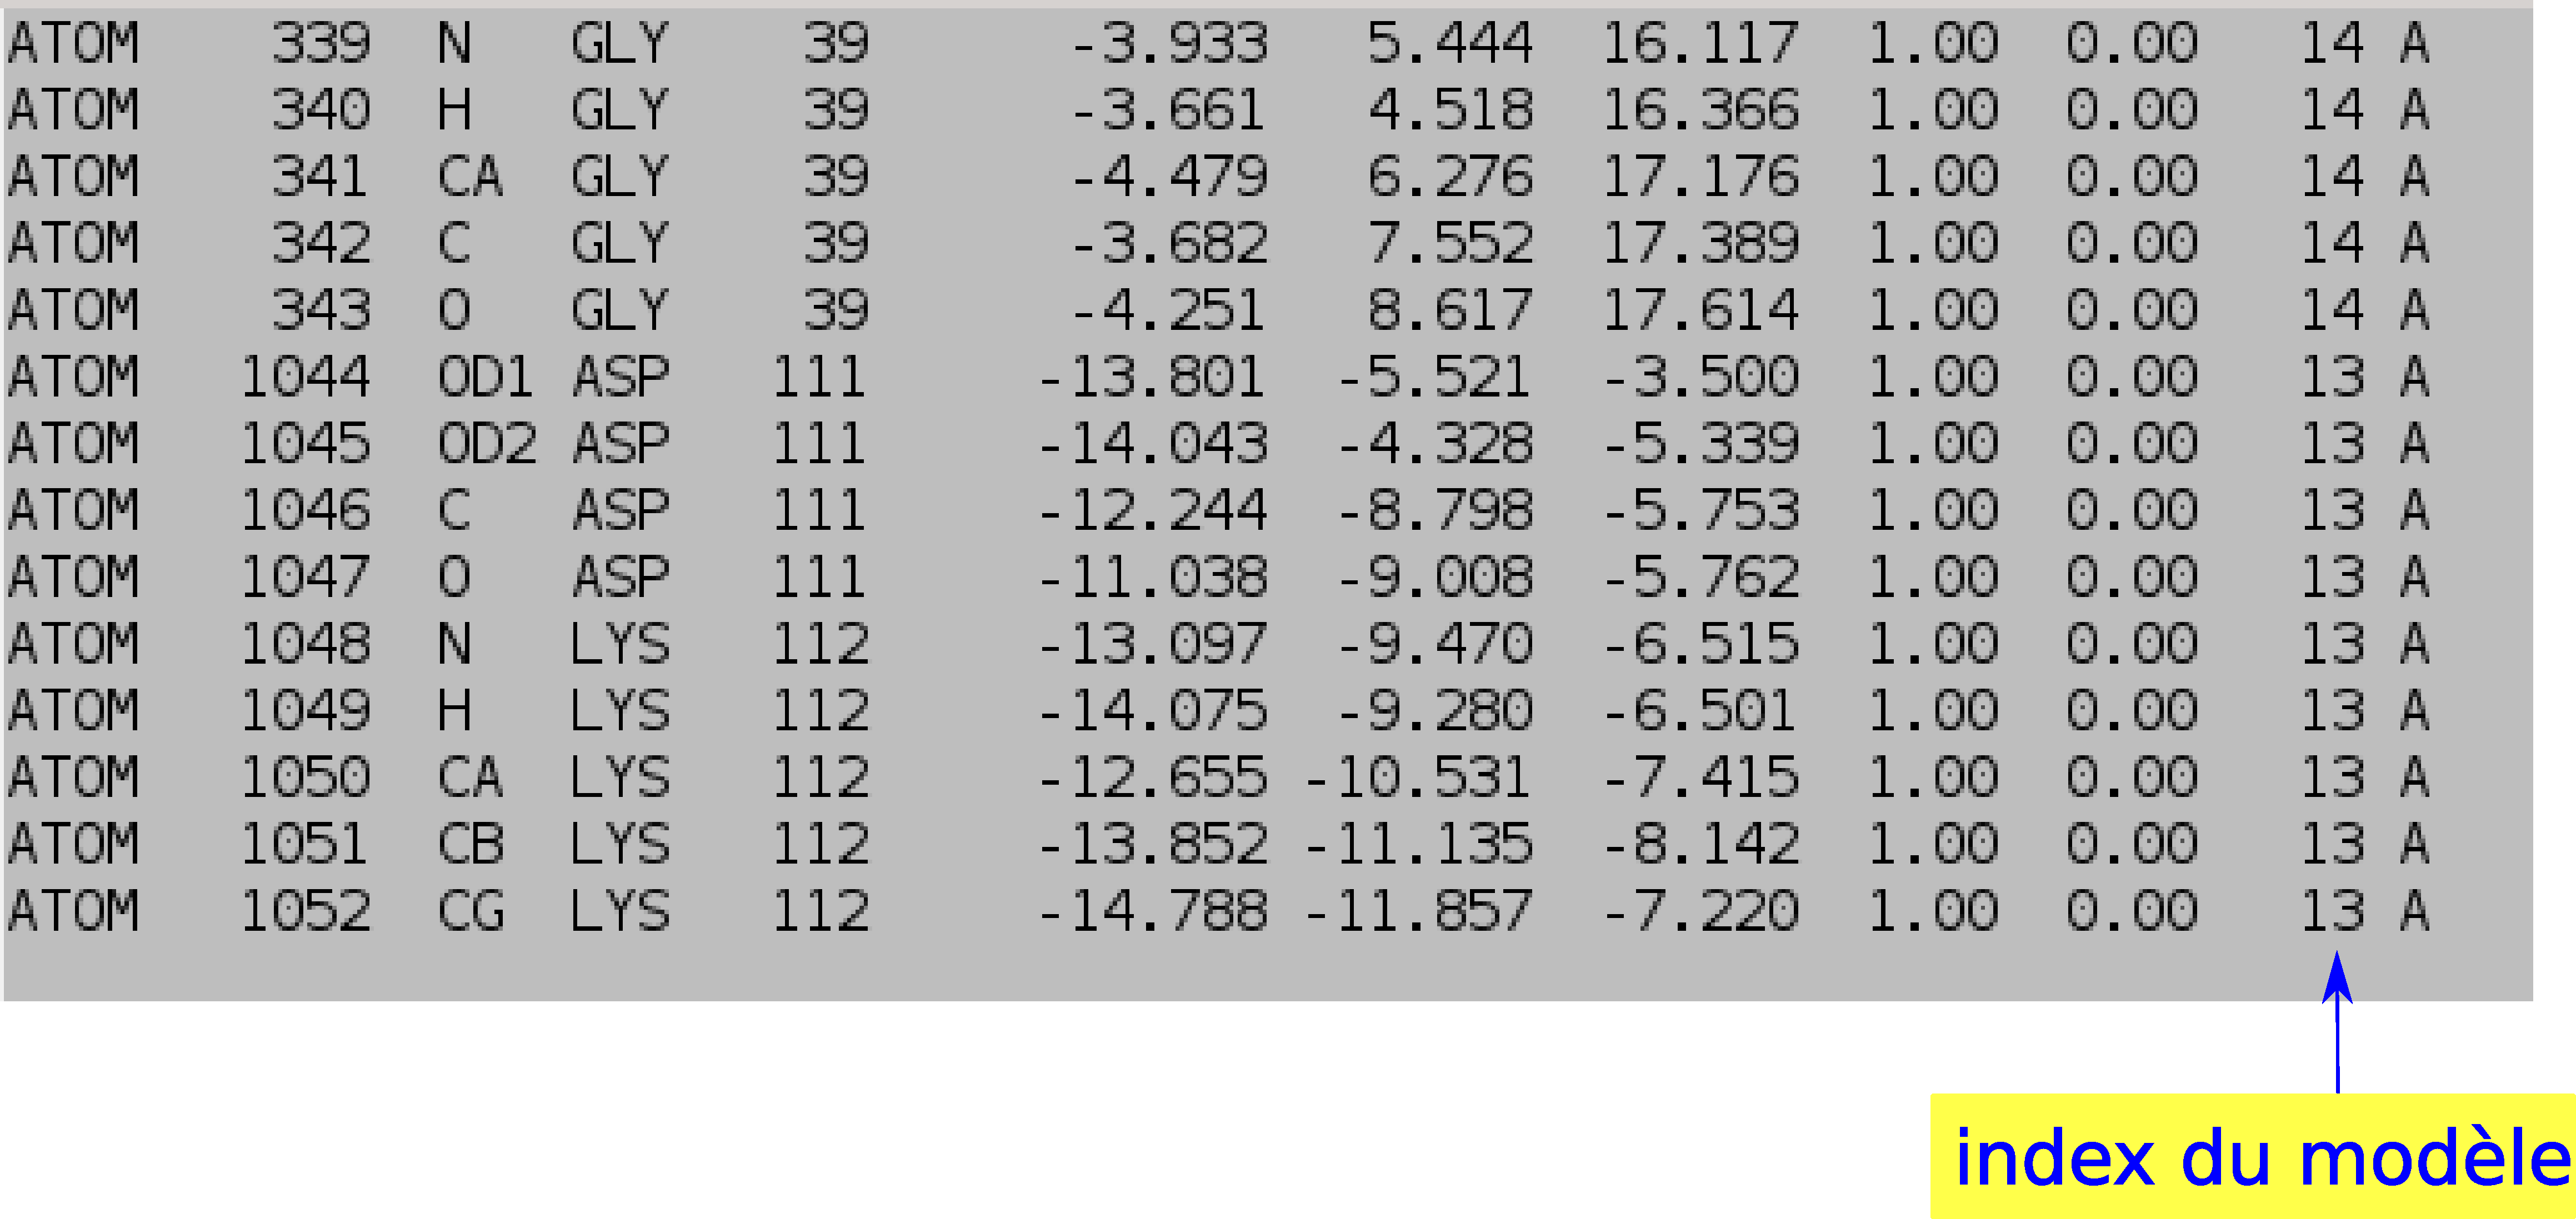
\includegraphics[width=13cm]{figure/PDB.pdf} 
     \end{tabular}     
     \caption{\textbf{Exemple de fichier PDB avec déclaration de 3 modèles.} L'avant-dernière colonne contient l'index des modèles. Par exemple, il y a un modèle pour GLY à la position 39 du segment A et un autre pour ASP, position 111, segment A.}
\label{fig:PDB}
   \end{figure}
 
L'utilisateur ne manipule que les modèles; les resclass n'apparaissent ni dans les fichiers d'entrée/sortie ni dans les commandes. Un modèle se déclare par des lignes ATOM d'un fichier PDB. Il y a deux possibilités de lecture des modèles. La commande:\\
\verb!coor disp=model @file.pdb!\\
ajoute chaque modèle de file.pdb dans un tableau en mémoire. Un nombre est lu à la colonne 67-71, il représente l'indice du modèle pour une resclass. Le lien avec la resclass se fait par la liste des atomes contenant l'indice, voir un exemple à la figure \ref{fig:PDB}. La commande:\\
\verb!coor disp=model @file.pdb push=true!\\
ajoute un seul modèle par resclass. L'indice d'un modèle n'est pas lu, mais calculé comme le plus grand indice existant plus un. 
La copie de modèle se fait par la commande:\\
\verb!coor copy from=A to=B idx=i=j end!\\
avec \verb!A! et \verb!B!  pouvant prendre les valeurs \verb!main!, \verb!comp!, \verb!xref! ou \verb!model!.
Le mot \verb!idx=i=j! n'est pas obligatoire. Par défaut, si \verb!from=model! alors \verb!idx=1! et si \verb!to=model! le nouvel indice créé sera le plus grand indice plus un. L'ancienne syntaxe est toujours supportée. La commande:\\ 
\verb!write coor sele=(resid $1 and resn $aa1) from=model output=new.pdb end!\\
imprime les modèles de chacune des resclass définies par la sélection dans un fichier PDB. On écrit une ligne par atome de la resclass avec l'indice du modèle, pour tous les modèles. 
Il est possible de limiter l'impression à un seul modèle $i$ par une commande du type:\\
\verb!write coor from=model idx=i output=new.pdb end!\\

\section{OpenMP pour le REMC}
\subsection{Présentation d'OpenMP}

Pour l'implémentation de l'algorithme \og Replica Exchange Monte Carlo\fg nous devons paralléliser la partie Monte-Carlo de proteus. Nous nous orientons vers une programmation à mémoire partagé. Dans ce domaine, l'interface de programmation OpenMP pour \og Open Multi-Processing\fg  offre un standard mature, bien supporté par les compilateurs C/C++ et simple à mettre en œuvre. Il s'agit d'une spécification qui décrit une collection de directives au compilateur, une bibliothèque de routines et un ensemble de variables d'environnement. Le principe est d'ajouter à un code existant des directives pour définir:
\begin{itemize}
\item les instructions à exécuter en parallèle (création de fils d'exécution); On parle de région parallèle dans le code.
\item les situations de synchronisations entre fils d'exécution
\item le statut des variables (partagé entre fils, privé, etc.) 
\end{itemize} 
La bibliothèque OpenMP permet la configuration de l'exécution et son contrôle par un ensemble de fonctions et de macros. Il existe des fonctions qui gèrent le nombre de fils d'exécution, qui fixent la politique de l'ordonnancement, qui retournent un identifiant du fil d'exécution, etc. La définition de la macro \_OPENMP garantit la compatibilité de l'exécutable.

Les variables d'environnement contrôlent les mêmes informations que les fonctions OpenMP. Elles doivent être définies avant l'exécution. Elles sont prises en compte avec une priorité plus faible que les fonctions de la bibliothèque, elles-mêmes de priorité plus faible que les directives en cas de conflit.

   \begin{figure}[!htbp]
     \centering
     \begin{tabular}{c}
       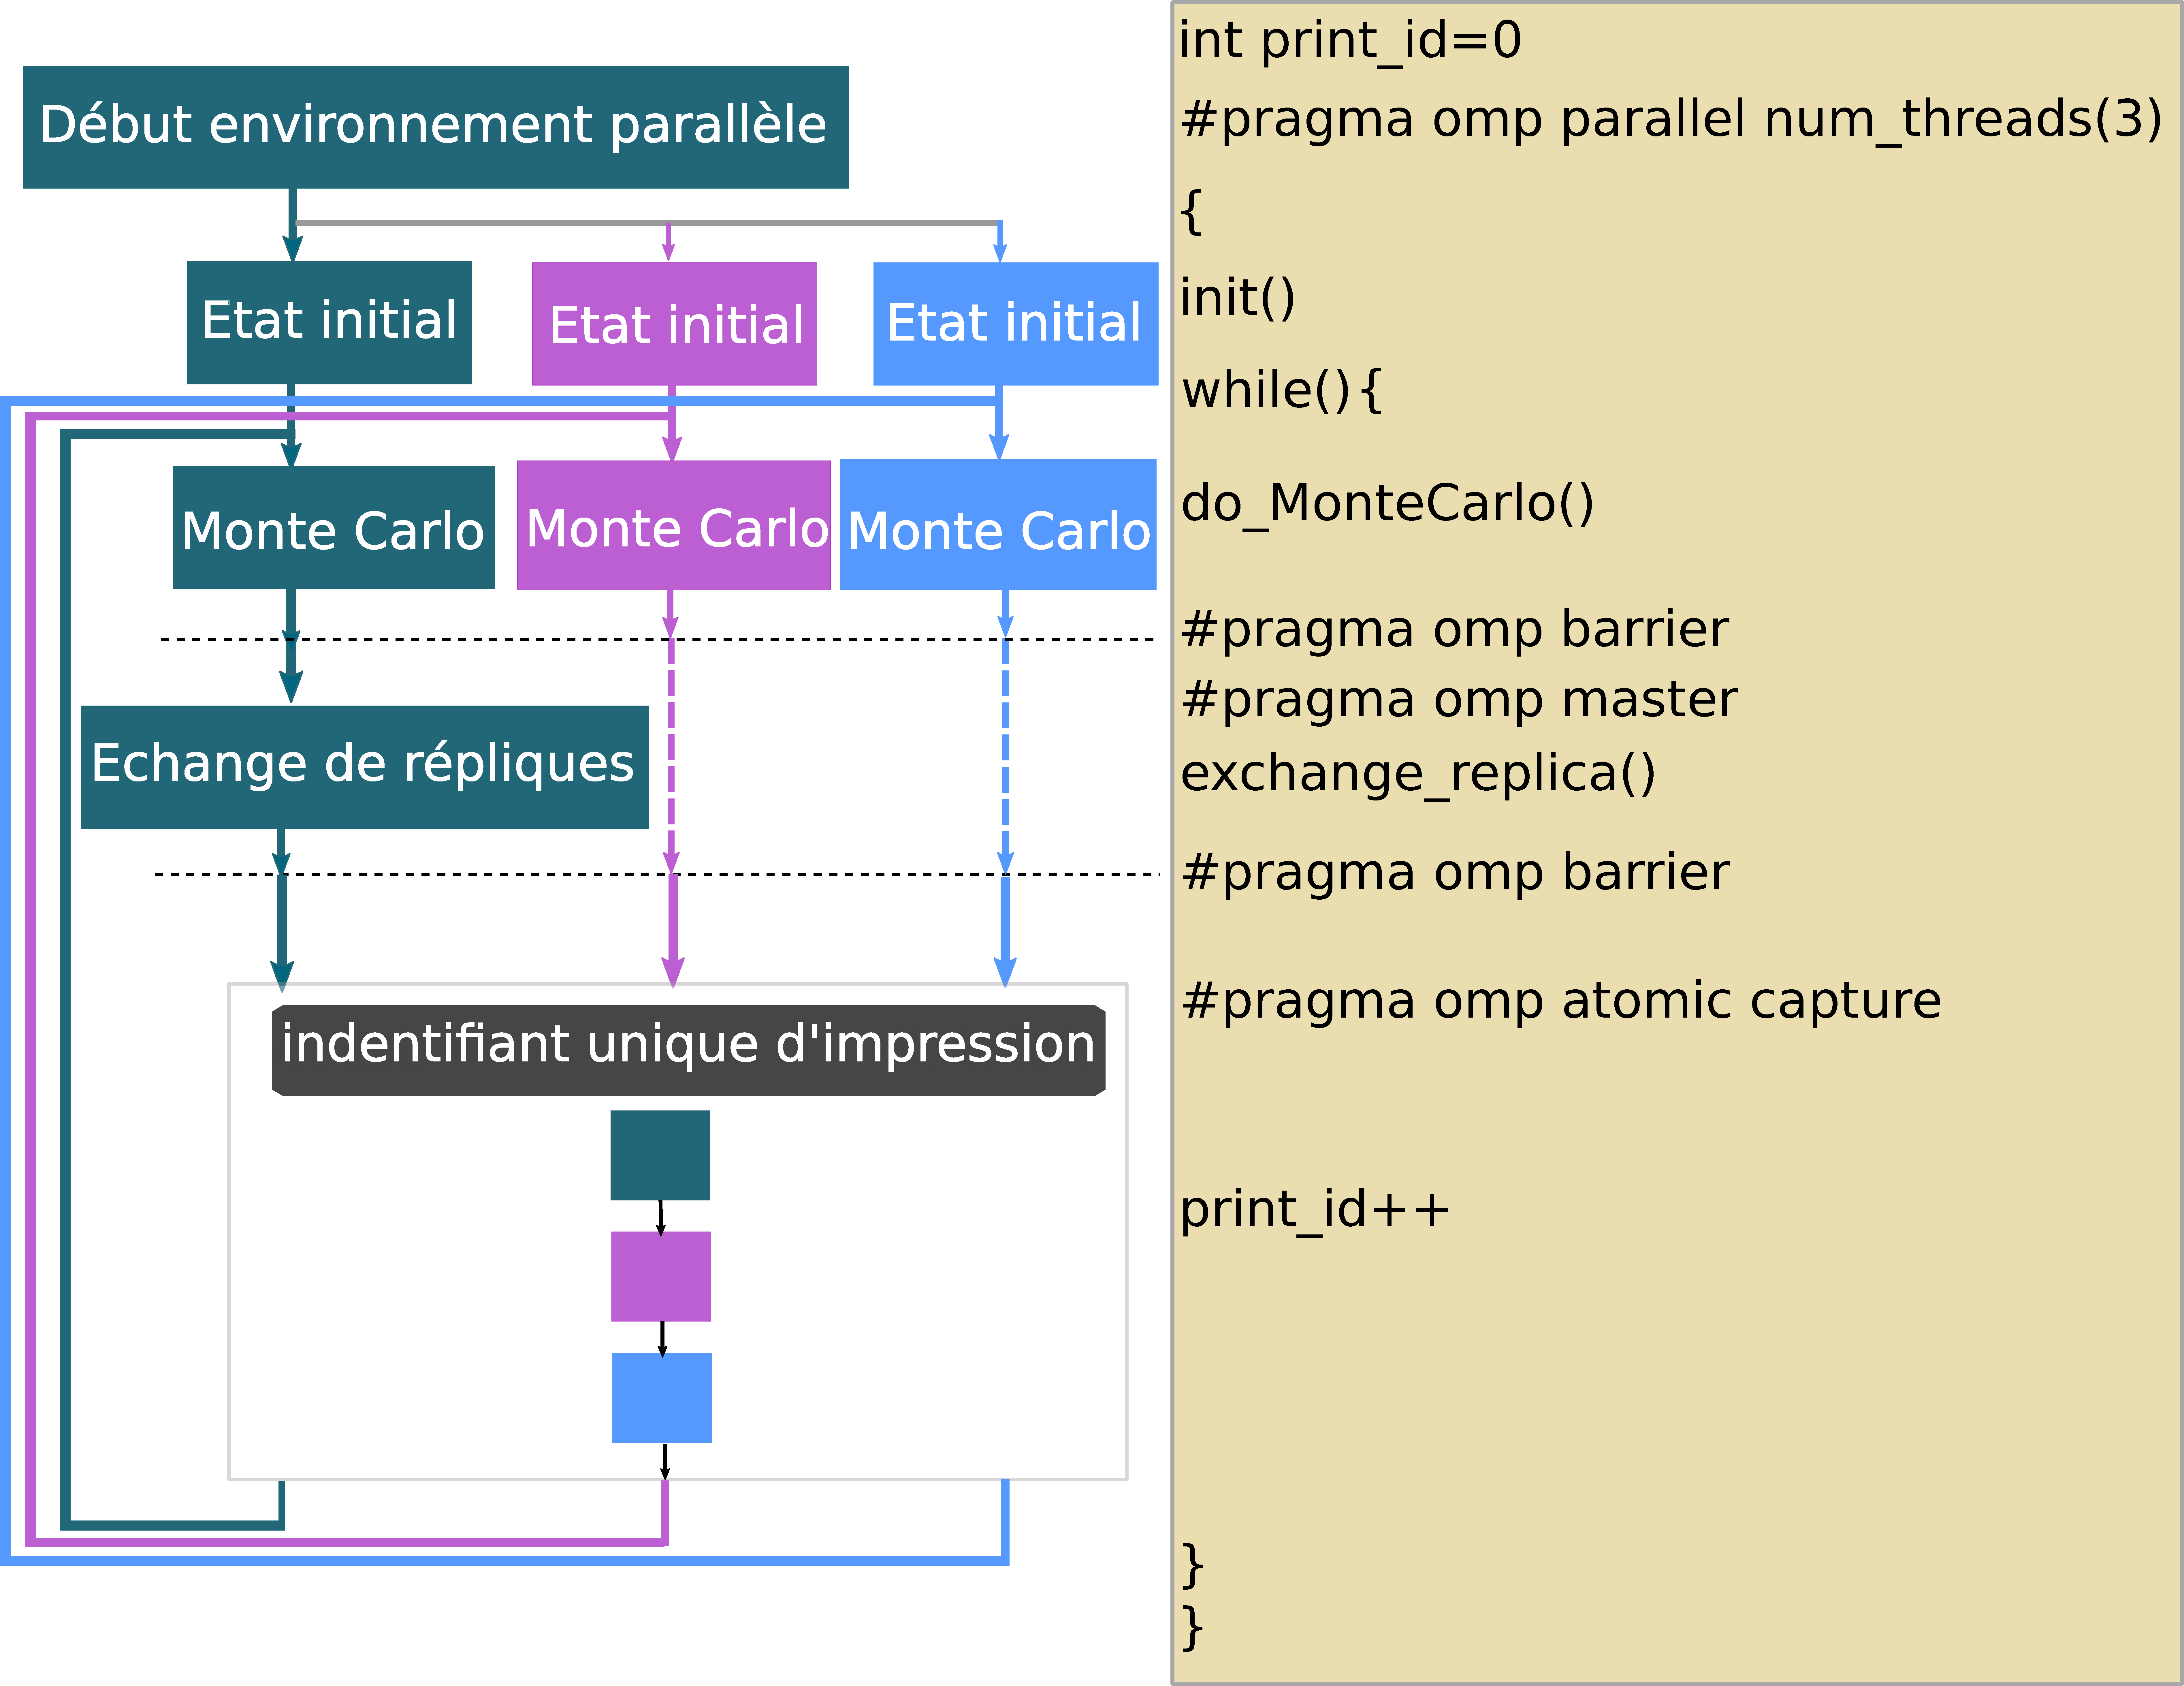
\includegraphics[width=14cm]{figure/openMP.pdf} 
     \end{tabular}     
     \caption{\textbf{La correspondance entre les directives OpenMP à droite et le comportement des fils d'exécution à gauche sur un REMC simplifié.} Sont schématisés, la création d'une région parallèle, deux synchronisations (les lignes pointillées à gauche), une région exécutée uniquement par un fil maître, une affectation séquentielle. }
\label{fig:openMP}
   \end{figure}

En entrant dans une région parallèle, le fil courant crée les autres fils. Il possède un statut particulier, il devient le fil maître. Les autres fils se terminent avec la région parallèle; le maître continue son exécution. Tous les fils ont accès à la même mémoire partagée, notamment aux variables définies avant la région parallèle. La déclaration d'une variable dans une région parallèle engendre la création d'une variable pour chaque fil accessible uniquement par lui. 
   

\subsection{REMC dans proteus}

Comme nous l'avons vu à la section \ref{REMC}, l'algorithme REMC considère plusieurs simulations indépendantes d'un même système. Cela fait de lui un algorithme bien adapté à la programmation parallèle. Deux points demandent une attention particulière: l'échange de répliques et la création de l'identifiant unique d'impression, voir \ref{proteusIO}. Le schéma général de REMC dans proteus est présenté à la figure \ref{fig:openMP}. Une région parallèle est initiée par la directive \og \#pragma omp parallel\fg: les différents marcheurs sont créés. Chacun réalise une trajectoire de type MC jusqu'à un nombre de pas multiple de la période d'échange. A priori l'avancée des marcheurs n'est pas simultanée. Donc une directive \og \#pragma omp barrier\fg est placée avant le test d'échange, elle garantit que chacun a effectué le bon nombre de pas. Une fois tous les marcheurs bloqués par cette directive, ils sont libérés. La directive \og \#pragma omp master\fg dédie l'exécution du test et de l'échange de répliques au seul marcheur maître. Pour empêcher les autres de marcher avant un échange éventuel, une seconde directive \og barrier\fg est placée après les instructions d'échanges.

Tout au long d'une trajectoire, des séquences-conformations sont imprimées. Pour faciliter le post-traitement, un identifiant unique sur toute l'exécution est attribué à chacune. Pour que tous les marcheurs puissent l'incrémenter, l'index qui sert d'identifiant est déclaré comme variable partagée. Pour garantir que chaque passage sur cette instruction retourne une valeur unique, une directive \og \#pragma omp atomic capture \fg est utilisée. Pour terminer cette section, nous donnons deux représentations graphiques du comportement des marcheurs REMC dans proteus à la figure \ref{fig:proteusREMC}.  

   \begin{figure}[!htbp]
     \centering
     \begin{tabular}{c}
       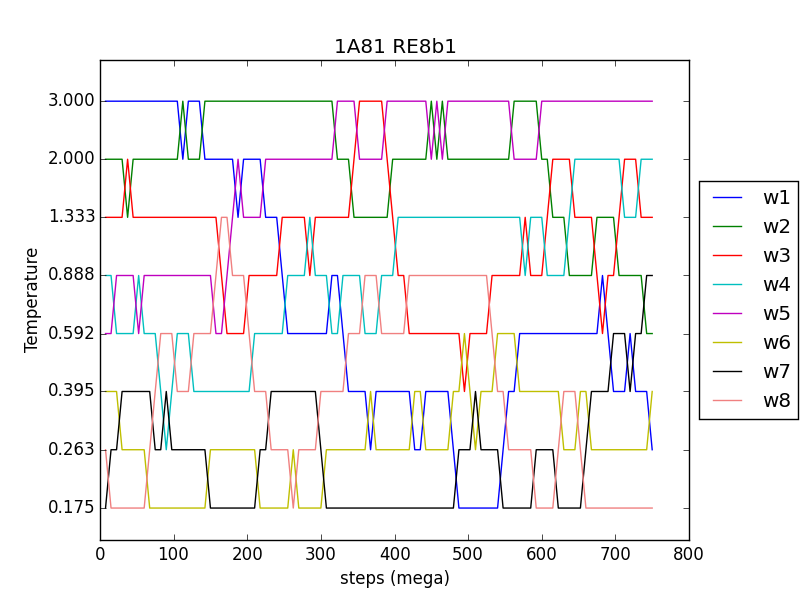
\includegraphics[width=12cm]{figure/re8_Ttraj.png}  \\
       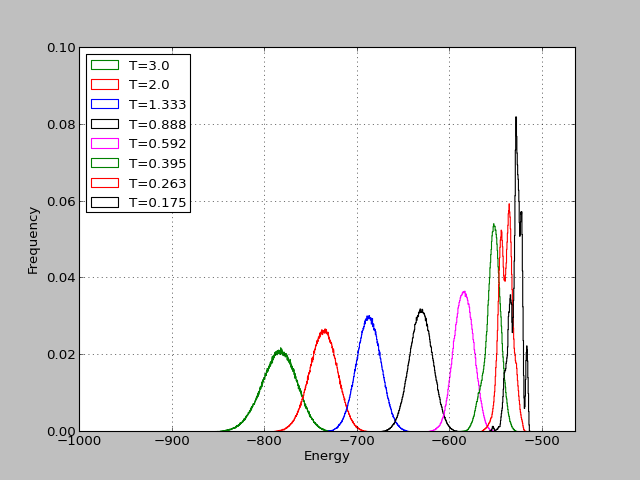
\includegraphics[width=12cm]{figure/re8_distri.png} \\
     \end{tabular}     
     \caption{\textbf{Comportement de proteus pour un REMC à huit marcheurs.} En haut, la trajectoire des marcheurs dans l'ensemble des huit températures. En bas, la distribution des énergies par marcheurs. On peut imaginer la distribution cumulée des marcheurs et remarquer que son graphe serait proche de celle d'une distribution de Boltzmann}
\label{fig:proteusREMC}
   \end{figure}
   

\section{Amélioration de la fonction d'acceptation MC}

Une amélioration a été apportée à la fonction d'acceptation MC de proteus. Pour réaliser une mutation du type $t$ vers $t'$, nous effectuons un changement de type d'acide aminé dans la structure repliée et le changement inverse dans la structure dépliée, voir la section \ref{sec:Phy}. La probabilité d'une mutation est donc le produit de la probabilité de choisir $t'$ par la probabilité de choisir une structure repliée particulière avec $t'$ et une structure dépliée particulière avec $t$. Dans proteus, ces changements sont sélectionnés par tirage aléatoire uniforme sur l'ensemble des états possibles. 

Se pose alors la question des états possibles des chaînes latérales à l'état déplié. Plusieurs points de vue sont possibles. On peut considérer qu'il existe autant de rotamères à l'état déplié qu'à état replié et qu'ils ont tous la même énergie. Cette possibilité a l'avantage de rendre la probabilité de mutation symétrique, c'est-à-dire que le passage du type $t$ vers $t'$ est aussi probable que le passage de $t'$ vers $t$. Mais elle a l'inconvénient d'être peu réaliste parce que les rotamères sont les positionnements préférentiels à l'état replié et non à l'état déplié. Nous avons fait évoluer proteus vers un autre point de vue, en considérant qu'une chaîne latérale à l'état déplié n'a qu'un seul rotamère dominant. Cela induit une dissymétrie dans la probabilité de sélection qui est corrigée par une probabilité d'acceptation du type de l'équation \ref{eq:Hasting}. Cette nouvelle probabilité d'acceptation est décrite en détail en \vref{eq:rule}.

\section{Nouveau système de déplacements}
\label{sec:newmove}
Le système de déplacements expliqué en \ref{sub:MC_move}  souffre de certaines rigidités. Il ne permet pas de distribuer les modifications selon les positions dans la chaîne polypeptidique. Il n'est pas possible de répartir alternativement les mouvements entre mutations et changement de rotamères.

Alors, nous introduisons deux nouvelles balises. La première permet la définition de deux poids à chaque position (dupliquée ou non). Le premier poids pondère la sélection d'une position lors d'une mutation, l'autre pondère la sélection d'une position lors d'un changement de rotamères:\\
\verb!<Position_Weights>! \\
\verb!Rot 489 0.50 ! \\
\verb!Rot 495 490-493 0.05 ! \\
\verb!Mut 489-491  G2.492 G3.489-491 0.052 ! \\
\verb!</Position_Weights>! \\
Les poids sont ensuite normalisés avant d'être utilisés lors de la sélection de positions. Ainsi, lorsque proteus prépare un changement de rotamère pendant la modification de la première position, la position $489$ a dix fois plus de chance d'être modifiée que $495$.

La balise \verb!<Step_Definition_Proba>! permet la construction en termes de probabilité du mouvement effectué à chaque pas. La syntaxe est la suivante:\\
\verb!<Step_Definition_Proba>! \\
\verb!Rot 1.0! \\
\verb!Mut Mut 0.1! \\
\verb!</Step_Definition_Proba>! \\
Chaque ligne à l'intérieur de la balise définit une forme de pas. Le nombre à la fin de la ligne fixe la probabilité du choix par proteus de cette forme. Les probabilités sont normalisées avant de début de la simulation. Ici, pour un pas quelconque d'une trajectoire, le changement de rotamère est choisi avec la probabilité $\frac{10}{11}$ et une double mutation est choisi avec la probabilité à $\frac{1}{11}$. Le choix de la seconde position à modifier se fait, comme précédemment, par un tirage uniforme sur l'ensemble des voisins de la première position.


\section{Label}
Dans certaines situations, le fichier de configuration de proteus peut devenir particulièrement grand. C'est le cas par exemple lorsque les énergies de références y sont définies. En effet, cela nécessite la déclaration d'une énergie pour chaque type d'acide aminé à chaque position de la chaîne polypeptidique du système étudié. Pour simplifier certaines déclarations, la nouvelle balise \verb!<Label>! permet de définir un alias sur un ensemble de mots. La syntaxe est la suivante:\\
\verb!<Label>! \\
\verb!exposed 11 15 17 19 ! \\
\verb!buried  12 13 14 16 18 20 21 ! \\
\verb!</Label>! \\
les labels \og exposed \fg et \og exposed \fg peuvent alors être utilisés de la façon suivante:\\
\verb!<Ref_Ener>! \\
\verb!CYS exposed  -1.09 ! \\
\verb!CYS exposed   2.60! \\
\verb!TYR buried   -4.34! \\
\verb!TYR buried   -1.92! \\
\verb!</Ref_Ener>! \\
cela définit les énergies de références pour CYS et TYR pour toutes les positions des deux ensembles.


\section{Allocation variable de la matrice}

Jusqu'à présent, proteus chargeait en mémoire la matrice d'énergie au début de son exécution. Avec l'introduction du GB/FDB la taille des données d'énergie peut être multiplié par un facteur huit environ. Afin de réduire l'usage de la mémoire, la dernière version du programme prend en compte les restrictions de l'espace de recherche déclarées dans le fichier de configuration pour limiter le chargement des énergies à celles nécessaires à l'exploration.  

\clearpage


%%% Local Variables:
%%% mode: latex
%%% TeX-master: "../these"
%%% End:
